\section{Introduction}

When modeling high-dimensional data where the number of features~(\(p\)) exceeds the number
of observations~(\(n\)), it is impossible to apply classical statistical models such as
standard linear regression since the design matrix \(\mat X\) is no longer of full rank. A
common remedy to this problem is to \emph{regularize} the model by adding a penalty term to
the objective that punishes models with large coefficients. The resulting problem takes the
following form:
\begin{equation}
  \label{eq:general-objective}
  \operatorname*{minimize}_{\beta_0 \in \mathbb{R},\vec{\beta} \in \mathbb{R}^p} g(\beta_0, \vec{\beta}; \mat X, \vec y) + h(\vec\beta),
\end{equation}
%
where \(\vec y\) is the response vector, \(\mat X\) the design matrix, \(\beta_0\) the
intercept, and \(\bm{\beta}\) the coefficients. Furthermore, \(g\) is a data-fitting
function that attempts to optimize the fit to the data and \(h\) is a penalty that depends
only on \(\bm{\beta}\). Two common penalties are the \(\ell_1\) norm and squared \(\ell_2\)
norm penalties, which if \(g\) is the standard ordinary least-squares objective, represent
the lasso~\citep{tibshirani1996,santosa1986,donoho1994} and ridge (Tikhonov) regression
respectively.

These penalties depend on the magnitudes of the coefficients, which means that they are
sensitive to the scales of the features in \(\mat X\). To avoid this, it is common to
\emph{normalize} the features before fitting the model by shifting and scaling each feature
by some measures of their locations and scales, respectively. For some problems it is
possible to arrive at these measures by contextual knowledge of the data at hand. In most
cases, however, they must be estimated. A popular strategy is to use the mean and standard
deviation of each feature as location and scale factors respectively, which is called
\emph{standardization}.

The choice of normalization may, however, have consequences for the estimated model. As a
first example of this, consider \Cref{fig:realdata-paths}, which displays the
regularization paths for the lasso\footnote{The estimated coefficients of the lasso as the
  penalty strength is varied from a large-enough value for all coefficients to be zero to a
  low value at which the model is almost saturated.} for four datasets:
\data{housing}~\citep{harrison1978}, \data{a1a}~\citep{becker1996,platt1998},
\data{triazines}~\citep{king1995,hirst1994}, and \data{w1a}~\citep{platt1998}, and two
types of normalization.

In the figure, we have colored the lines corresponding to features that were among the
first five to enter the model in either of the two type of normalization schemes. Note that
the choice of normalization result in different sets of features being selected as well as
different coefficient estimates. This is especially striking in the case of
\data{triazines} and \data{w1a}.

\begin{figure}[bpt]
  \centering
  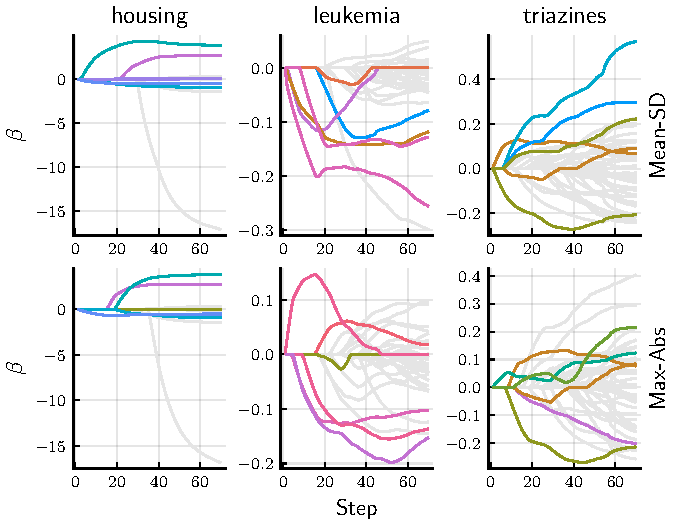
\includegraphics[]{realdata_paths.pdf}
  \caption{%
    Lasso paths for real datasets using two types of normalization:
    standardization and maximum absolute value normalization (max--abs). For
    each dataset, we have colored the coefficients if they were among the first
    five to become non-zero under either of the two normalization schemes.
    The \(x\)-axis shows the steps along the regularization path and
    the \(y\)-axis the estimated coefficients normalized by the
    maximum magnitude of the coefficients in each case. See
    \Cref{sec:data-summary} for more information about datasets used here.
  }
  \label{fig:realdata-paths}
\end{figure}

To illustrate this further, we show the estimated coefficients for the same datasets after
having fitted the lasso with a penalty strength (\(\lambda\)) set from 5-fold
cross-validation repeated 5 times on a 50\% train set split. The results are shown in
\Cref{tab:realdata-cv-coefs}. We see that the estimated coefficients on the test set are
different between the two cases, especially for the \data{triazines} datasets, where the
two normalization schemes disagree completely.

\begin{table}[htpb]
  \centering
  \caption{
    Estimated lasso coefficients on test sets, with \(\lambda\) set from 5-fold
    cross-validation repeated 5 times. \(\hat{\bm{\beta}}_\text{std}\) and
    \(\hat{\bm{\beta}}_\text{max--abs}\) show the
    coefficients based on normalizing the design matrix with standardization and
    maximum absolute value (max--abs) normalization respectively. We show the five largest
    coefficients (in magnitude) for the standardization case and the respective
    coefficients for the max--abs case. In each case, we present the coefficients
    on the original scale of the features.
    See \Cref{sec:data-summary} for more
    information about these datasets.
  }
  \label{tab:realdata-cv-coefs}
  \begin{tabular}{
      S[table-format=-1.2,round-mode=figures,round-precision=2]
      S[table-format=-1.2,round-mode=figures,round-precision=2]
      S[table-format=-1.2,round-mode=figures,round-precision=2]
      S[table-format=-1.4,round-mode=figures,round-precision=2]
      S[table-format=1.3,round-mode=figures,round-precision=2]
      S[table-format=1.1,round-mode=figures,round-precision=2]
      S[table-format=1.1,round-mode=figures,round-precision=2]
      S[table-format=1.2,round-mode=figures,round-precision=2]
    }
    \toprule
    \multicolumn{2}{c}{\data{housing}} & \multicolumn{2}{c}{\data{a1a}}         & \multicolumn{2}{c}{\data{triazines}} & \multicolumn{2}{c}{\data{w1a}}                                                                                                                                                                   \\
    \cmidrule(rl){1-2}
    \cmidrule(rl){3-4}
    \cmidrule(rl){5-6}
    \cmidrule(rl){7-8}
    {\(\hat{\bm{\beta}}_\text{std}\)}  & {\(\hat{\bm{\beta}}_\text{max--abs}\)} & {\(\hat{\bm{\beta}}_\text{std}\)}    & {\(\hat{\bm{\beta}}_\text{max--abs}\)} & {\(\hat{\bm{\beta}}_\text{std}\)} & {\(\hat{\bm{\beta}}_\text{max--abs}\)} & {\(\hat{\bm{\beta}}_\text{std}\)} & {\(\hat{\bm{\beta}}_\text{max--abs}\)} \\
    \midrule
    -0.6309                            & -0.675004                              & 0.542532                             & 0.536762                               & 0.17369                           & 0.0                                    & 1.80033                           & 0.0                                    \\
    -1.38393                           & -0.779929                              & 0.327537                             & 0.523057                               & 0.0691224                         & 0.0                                    & 1.78789                           & 0.78455                                \\
    0.265659                           & 0.0                                    & -0.388699                            & -0.514664                              & 0.0284156                         & 0.0                                    & 1.78348                           & 0.630671                               \\
    -0.987113                          & -0.335828                              & 0.308715                             & 0.320916                               & 0.0706408                         & 0.0                                    & 1.44741                           & 0.07977                                \\
    2.77031                            & 3.06118                                & 0.175958                             & 0.23103                                & 0.0293775                         & 0.0                                    & 1.65553                           & 0.0                                    \\
    \bottomrule
  \end{tabular}
\end{table}

In spite of this apparent connection between normalization and regularization, there has so
far been almost no research on the topic. And in its absence, the choice of normalization
is typically motivated by computational concerns or by being ``standard''. This is
problematic since the effects of normalization are unknown and because there exists no
natural choice for many types of data. In particular, there is no obvious choice for binary
features (where each observation takes either of two values). In this paper we begin to
bridge this knowledge gap by studying normalization in the context of three particular
cases of the regularized problem in \Cref{eq:general-objective}: the lasso, ridge, and
elastic net~\citep{zou2005}. The latter of these, the elastic net, is a generalization of
the previous two, and is represented by the following optimization problem:
%
\begin{equation}
  \label{eq:elastic-net}
  \operatorname*{minimize}_{\beta_0 \in \mathbb{R},\vec{\beta} \in \mathbb{R}^p} \frac{1}{2} \lVert \vec y - \beta_0 - \tilde{\mat{X}}\vec{\beta} \rVert^2_2  + \lambda_1 \lVert \vec\beta \rVert_1 + \frac{\lambda_2}{2}\lVert \vec \beta \rVert_2^2,
\end{equation}
%
where setting \(\lambda_1 = 0\) results in ridge regression and setting \(\lambda_2 = 0\)
results in the lasso. Our focus in this paper is on binary data and we pay particular
attention to the case when they are imbalanced, that is, have relatively many ones or
zeroes. In this scenario, we demonstrate that the choice of normalization directly
influences the estimated coefficients and that this effect depends on the particular
combination of normalization and regularization.

Our key contributions are:
\begin{enumerate}
  \item We reveal that class balance in binary features directly affects lasso, ridge, and elastic
        net estimates, and show that scaling binary features with standard deviation (ridge) or
        variance (lasso) mitigates these effects at the cost of increased variance. In our
        theoretical work~(\Cref{sec:theory-binary-features}), we show that this relationship holds
        even in the simple case of orthogonal features, and also provide empirical evidence that
        these findings extend to much more general settings~(\Cref{sec:experiments}).
  \item For mixed data designs, we demonstrate that normalization choice implicitly determines how
        regularization affects binary versus continuous features~(\Cref{sec:mixed-data}).
  \item For interaction features, we show that a common alternative to normalizing the interaction
        feature leads to biased estimates and provide an alternative that mitigates this
        problem~(\Cref{sec:interactions}).
\end{enumerate}

Collectively, our results demonstrate that normalization is not merely a preprocessing step
but rather an integral component of the model that requires careful consideration based on
data characteristics and the chosen regularization approach.
